\chapter{CTF 基础知识}\index{CTF 基础知识}
\section{CTF 简介}
% \setlength{\parindent}{2em}
\subsection{概述}
\indent \setlength{\parindent}{2em}
\indent CTF(Capture The Flag)中文一般译作夺旗赛,在网络安全领域中指的是网络安全技术人员之间进行技术竞技的一种比赛形式。CTF起源于1996年DEFCON全球黑客大会,以代替之前黑客们通过互相发起真实攻击进行技术比拼的方式。发展至今,已经成为全球范围网络安全圈流行的竞赛形式,2013年全球举办了超过五十场国际性CTF赛事。而DEFCON作为CTF赛制的发源地,DEFCON CTF也成为了目前全球最高技术水平和影响力的CTF竞赛,类似于CTF赛场中的“世界杯”。

\indent CTF 为团队赛,通常以三人为限,要想在比赛中取得胜利,就要求团队中每个人在各种类别的题目中至少精通一类,三人优势互补,取得团队的胜利。同时,准备和参与 CTF 比赛是一种有效将计算机科学的离散面、聚焦于计算机安全领域的方法。

\subsection{赛事介绍}
\indent \setlength{\parindent}{2em}

\indent CTF是一种流行的信息安全竞赛形式,其英文名可直译为“夺得Flag”,也可意译为“夺旗赛”。其大致流程是,参赛团队之间通过进行攻防对抗、程序分析等形式,率先从主办方给出的比赛环境中得到一串具有一定格式的字符串或其他内容,并将其提交给主办方,从而夺得分数。为了方便称呼,我们把这样的内容称之为“Flag”。

\indent CTF竞赛模式具体分为以下三类:
\begin{itemize}
    \item \textbf{解题模式(Jeopardy)} 
    \indent 在解题模式CTF赛制中,参赛队伍可以通过互联网或者现场网络参与,这种模式的CTF竞赛与ACM编程竞赛、信息学奥赛比较类似,以解决网络安全技术挑战题目的分值和时间来排名,通常用于在线选拔赛。题目主要包含逆向、漏洞挖掘与利用、Web渗透、密码、取证、隐写、安全编程等类别。
    
    \item \textbf{攻防模式(Attack-Defense)}
    \indent 在攻防模式CTF赛制中,参赛队伍在网络空间互相进行攻击和防守,挖掘网络服务漏洞并攻击对手服务来得分,修补自身服务漏洞进行防御来避免丢分。攻防模式CTF赛制可以实时通过得分反映出比赛情况,最终也以得分直接分出胜负,是一种竞争激烈,具有很强观赏性和高度透明性的网络安全赛制。在这种赛制中,不仅仅是比参赛队员的智力和技术,也比体力(因为比赛一般都会持续48小时及以上),同时也比团队之间的分工配合与合作。
    
    \item \textbf{混合模式(Mix)}
    \indent 结合了解题模式与攻防模式的CTF赛制,比如参赛队伍通过解题可以获取一些初始分数,然后通过攻防对抗进行得分增减的零和游戏,最终以得分高低分出胜负。采用混合模式CTF赛制的典型代表如iCTF国际CTF竞赛。
\end{itemize}


\subsection{题目类别}
\indent \setlength{\parindent}{2em}

\begin{itemize}
    \item Reverse
    \begin{itemize}
        \item 题目涉及到软件逆向、破解技术等,要求有较强的反汇编、反编译功底。主要考查参赛选手的逆向分析能力。
        \item 所需知识:汇编语言、加密与解密、常见反汇编工具
    \end{itemize}
    
    \item Pwn
    \begin{itemize}
        \item Pwn 在黑客俚语中代表着攻破,获取权限,在 CTF 比赛中它代表着溢出类的题目,其中常见类型溢出漏洞有整数溢出、栈溢出、堆溢出等。主要考查参赛选手对漏洞的利用能力。
        \item 所需知识:C,OD+IDA,数据结构,操作系统
    \end{itemize}
    
    \item Web
    \begin{itemize}
        \item Web 是 CTF 的主要题型,题目涉及到许多常见的 Web 漏洞,如 XSS、文件包含、代码执行、上传漏洞、SQL 注入等。也有一些简单的关于网络基础知识的考察,如返回包、TCP/IP、数据包内容和构造。有些题目环境比较接近真实环境,因此通过各种高质量Web题目可以迅速提高选手的安全技能。
        \item 所需知识:基础的web开发能力,一门脚本语言(PHP、Python)、JavaScript、数据库、网络协议等
    \end{itemize}
   
    \item Crypto
    \begin{itemize}
        \item 题目考察各种加解密技术,包括古典加密技术、现代加密技术甚至出题者自创加密技术,以及一些常见编码解码,主要考查参赛选手密码学相关知识点。通常也会和其他题目相结合。
        \item 所需知识:数论、现代密码学和一门编程语言(C或Python)
    \end{itemize}
    
    \item Misc
    \begin{itemize}
        \item Misc 即安全杂项,题目涉及隐写术、流量分析、电子取证、人肉搜索、数据分析、大数据统计等,覆盖面比较广,主要考查参赛选手的各种基础综合知识。
        \item 所需知识:常见隐写术工具、Wireshark 等流量审查工具、编码知识;此类题目知识繁杂,有时候更需要一个灵活的思路
    \end{itemize}
    
    \item Mobile(Android)
    \begin{itemize}
        \item 主要分为 Android 和 iOS 两个平台,以 Android 逆向为主,破解 APK 并提交正确答案。
        \item 所需知识:Java,Android 开发,常见工具
    \end{itemize}
\end{itemize}

\subsection{高质量的CTF比赛}
\indent \setlength{\parindent}{2em}

\indent 详见:
\begin{itemize}
    \item 国外比赛平台:\url{http://www.ctftime.org}
    \item 国内CTF评分网站:\url{https://www.ctfrank.org}
\end{itemize}


\subsection{竞赛小贴士}
\indent \setlength{\parindent}{2em}
\begin{itemize}
    \item 寻找团队
    \begin{itemize}
        \item 彼此激励24小时以上的连续作战
        \item 彼此分享交流技术与心得是最快的成长途径
        \item 强有力的团队可以让你安心专注于某一领域
        \item 在探索技术的道路上不会孤独
    \end{itemize}
    
    \item 有效训练
    \begin{itemize}
        \item 坚持不懈地训练是成为强者的必经途径
        \begin{itemize}
            \item wargame
            \item 经典赛题配合writeup加以总结
            \item https://github.com/ctfs 以赛代练,总结与分享
        \end{itemize}
    \end{itemize}
    \item wargame推荐
    \begin{itemize}
        \item 漏洞挖掘与利用(pwn)
        \begin{itemize}
            \item pwnable.kr
            \item \href{https://exploit-exercises.com}{https://exploit-exercises.com}
            \item \href{https://io.netgarage.org}{https://io.netgarage.org}
        \end{itemize}
        
        \item 逆向工程与软件破解(re)
        \begin{itemize}
            \item reversing.kr
            \item \href{http://crackmes.de}{http://crackmes.de}
        \end{itemize}
        
        \item web渗透(web)
        \begin{itemize}
            \item webhacking.kr
            \item \href{https://xss-game.appspot.com}{https://xss-game.appspot.com}
        \end{itemize}
        
        \item 综合类
        \begin{itemize}
            \item \href{http://overthewire.org/wargames}{http://overthewire.org/wargames}
            \item \href{https://w3challs.com}{https://w3challs.com}
            \item \href{https://chall.stypr.com/?chall}{https://chall.stypr.com/?chall}
            \item \href{https://pentesterlab.com}{https://pentesterlab.com}
        \end{itemize}
    \end{itemize}
\end{itemize}

\subsection{线下赛 AWD 模式概述}
\indent \setlength{\parindent}{2em}

\indent Attack With Defence,简而言之就是你既是一个 hacker,又是一个 manager。

\indent 比赛形式:一般就是一个 ssh 对应一个服务,可能是 web 也可能是 pwn,然后 flag 五分钟一轮,各队一般都有自己的初始分数,flag 被拿会被拿走 flag 的队伍均分,主办方会对每个队伍的服务进行 check,check 不过就扣分,扣除的分值由服务 check 正常的队伍均分。

\subsubsection{怎样拿到Flag}
\indent \setlength{\parindent}{2em}
\intent web 主要是向目标服务器发送 http 请求,返回 flag,bin 主要是通过 exploit 脚本读取 \verb+/home/username+ 下某个文件夹下的 \verb+flag+ 文件。

\subsubsection{Web 题目类型}\setlength{\parindent}{2em}
\begin{itemize}
    \item 出题人自己写的 CMS 或者魔改后的 CMS(注意最新漏洞、1day漏洞等)
    \item 常见(比如 Wordpress、Discuz!)或者不常见 CMS 等
    \item 框架型漏洞(CI等)
    \item \href{http://www.mamicode.com/info-detail-1590551.html}{如何在 CTF 中当搅屎棍}
    \item \href{http://bobao.360.cn/ctf/detail/169.html}{AWD 模式生存技巧}
    \item 能力:
    \begin{itemize}
        \item 漏洞反应能力
        \item 快速编写脚本
        \item web代码审计
        \item 心态放好,因为 web 比较容易抓取流量,所以即使我们被打,我们也可以及时通过分析流量去查看别的队伍的 payload,从而进行反打。
    \end{itemize}
    \item 脚本准备:一句话,文件包含,不死马、禁止文件上传等
    \item \textbf{警惕 web 弱口令,用最快的速度去补}
\end{itemize}


\subsubsection{Bin 题目类型}
\indent \setlength{\parindent}{2em}
\indent 大部分是 PWN,题目类型包括栈、堆、格式化字符串等等。

\indent 能力:
\begin{itemize}
    \item 迅速找到二进制文件的漏洞,迅速打 patch 的能力
    \item 全场打 pwn 的 exp 脚本编写
    \item 熟悉服务器运维,如果二进制分析遇到障碍难以进行,那就去帮帮 web 选手运维
    \item 尽快摸清楚比赛的 check 机制
    \item 看看现场环境是否可以提权,这样可以方便我们搞操作(如魔改libc等等)
\end{itemize}

\subsubsection{技巧}
\begin{itemize}
    \item 如果自己拿到 FB, 先用 NPC 服务器或者自己服务器测试,格外小心自己的 payload 不要被别的队伍抓取到, 写打全场的 exp 时,一定要加入混淆流量。
    \item 提前准备好 PHP 一句话木马等等脚本。
    \item 小心其他队伍恶意攻击使我们队伍机器的服务不能正常运行,因此一定要备份服务器的配置。
    \item 尽可能在不搞崩服务和绕过 check 的情况下,上 WAF,注意分析别人打过来的流量,如果没有混淆,可以大大加快我们的漏洞分析速度。
    \item 工具准备: 中国菜刀、 Nmap、Xshell、 合适的扫描器等。
    \item 如果自己丢分,心态不要崩。
    \item 不要忽视 Github 等平台,可能会有写好的 exp 可以用。
    \item 将 flag 的提交自动化。
\end{itemize}



\subsection{搭建CTF平台}
\indent \setlength{\parindent}{2em}
\indent 已经有现成开源平台供我们使用:
\indent \begin{itemize}
    \item \href{https://github.com/facebook/fbctf}{FBCTF} - The Facebook CTF is a platform to host Jeopardy and “King of the Hill” style Capture the Flag competitions.
    
    \item \href{https://github.com/CTFd/CTFd}{CTFd} - CTFd is a Capture The Flag in a can. It's easy to customize with plugins and themes and has everything you need to run a jeopardy style CTF.
    
    \item \href{https://github.com/cliffe/SecGen}{SecGen} - SecGen creates vulnerable virtual machines so students can learn security penetration testing techniques.
\end{itemize}

\subsection{参考}
\indent \setlength{\parindent}{2em}

\indent \href{https://baike.baidu.com/item/ctf/9548546}{https://baike.baidu.com/item/ctf/9548546}

\section{学习方法}
\indent \setlength{\parindent}{2em}
\indent \href{https://github.com/ryanhanwu/How-To-Ask-Questions-The-Smart-Way}{提问的智慧}

\section{Linux基础}
\setlength{\parindent}{2em}

\subsection{常用Linux命令}
\subsubsection{常用基础命令}
\begin{lstlisting}[language=bash, style=customStyleBashDark, caption=基础命令]
ls                  # 用来显示目标列表
cd [path]           # 用来切换工作目录
pwd                 # 以绝对路径的方式显示用户当前工作目录
man [command]       # 查看Linux中的指令帮助等信息
echo [string]       # 打印一行文本,参数“-e”可激活转义字符
cat [file]          # 连接文件并打印到标准输出设备上
less [file]         # 允许用户向前或向后浏览文字档案的内容
mv [file1] [file2]  # 对文件或目录重新命名,或者将文件从一个目录移到另一个目录
cp [file1] [file2]  # 复制文件到指定的目的文件或目录
rm [file]           # 可以删除一个目录中的一个或多个文件或目录
ps                  # 用于报告当前系统的进程状态
top                 # 实时查看系统的整体运行情况
kill                # 杀死一个进程
ifconfig            # 查看或设置网络设备
ping                # 查看网络上的主机是否工作
netstat             # 显示网络连接、路由表和网络接口信息
nc(netcat)          # 建立 TCP 和 UDP 连接并监听
su                  # 切换当前用户身份到其他用户身份
touch [file]        # 创建新的空文件
mkdir [dir]         # 创建目录
chmod               # 变更文件或目录的权限
chown               # 变更某个文件或目录的所有者和所属组
nano / vim / emacs  # 字符终端的文本编辑器
exit                # 退出 shell
|                   # 将一个命令的标准输出作为另一个命令的标准输入
\end{lstlisting}

\subsubsection{Bash 快捷键}
\indent \setlength{\parindent}{2em}
\begin{lstlisting}[language=bash, style=customStyleBashDark, caption=Bash快捷键]
Up(Down)          # 上(下)一条指令
Ctrl + c          # 终止当前进程
Ctrl + z          # 挂起当前进程,使用“fg”可唤醒
Ctrl + d          # 删除光标处的字符
Ctrl + l          # 清屏
Ctrl + a          # 移动到命令行首
Ctrl + e          # 移动到命令行尾
Ctrl + b          # 按单词后移(向左)
Ctrl + f          # 按单词前移(向右)
Ctrl + Shift + c  # 复制
Ctrl + Shift + v  # 粘贴
\end{lstlisting}
\indent 更多细节请查看:\href{https://ss64.com/bash/syntax-keyboard.html}{bash keyboard shortcuts}

\subsubsection{根目录结构}
\indent \setlength{\parindent}{2em}

\begin{lstlisting}[language=bash, style=customStyleBashDark, caption=目录结构]
$ uname -a
Linux manjaro 4.11.5-1-ARCH #1 SMP PREEMPT Wed Jun 14 16:19:27 CEST 2017 x86_64 GNU/Linux

$ ls -al /
drwxr-xr-x  17 root root  4096 Jun 28 20:17 .
drwxr-xr-x  17 root root  4096 Jun 28 20:17 ..
lrwxrwxrwx   1 root root     7 Jun 21 22:44 bin -> usr/bin
drwxr-xr-x   4 root root  4096 Aug 10 22:50 boot
drwxr-xr-x  20 root root  3140 Aug 11 11:43 dev
drwxr-xr-x 101 root root  4096 Aug 14 13:54 etc
drwxr-xr-x   3 root root  4096 Apr  8 19:59 home
lrwxrwxrwx   1 root root     7 Jun 21 22:44 lib -> usr/lib
lrwxrwxrwx   1 root root     7 Jun 21 22:44 lib64 -> usr/lib
drwx------   2 root root 16384 Apr  8 19:55 lost+found
drwxr-xr-x   2 root root  4096 Oct  1  2015 mnt
drwxr-xr-x  15 root root  4096 Jul 15 20:10 opt
dr-xr-xr-x 267 root root     0 Aug  3 09:41 proc
drwxr-x---   9 root root  4096 Jul 22 22:59 root
drwxr-xr-x  26 root root   660 Aug 14 21:08 run
lrwxrwxrwx   1 root root     7 Jun 21 22:44 sbin -> usr/bin
drwxr-xr-x   4 root root  4096 May 28 22:07 srv
dr-xr-xr-x  13 root root     0 Aug  3 09:41 sys
drwxrwxrwt  36 root root  1060 Aug 14 21:27 tmp
drwxr-xr-x  11 root root  4096 Aug 14 13:54 usr
drwxr-xr-x  12 root root  4096 Jun 28 20:17 var
\end{lstlisting}

\indent 由于不同的发行版会有略微的不同,我们这里使用的是基于 Arch 的发行版 Manjaro,以上就是根目录下的内容,我们介绍几个重要的目录:
\begin{itemize}
    \item \verb+/bin+、\verb+/sbin+:链接到 \verb+/usr/bin+,存放 Linux 一些核心的二进制文件,其包含的命令可在 shell 上运行。
    \item \verb+/boot+:操作系统启动时要用到的程序。
    \item \verb+/dev+:包含了所有 Linux 系统中使用的外部设备。需要注意的是这里并不是存放外部设备的驱动程序,而是一个访问这些设备的端口。
    \item \verb+/etc+:存放系统管理时要用到的各种配置文件和子目录。
    \item \verb+/etc/rc.d+:存放 Linux 启动和关闭时要用到的脚本。
    \item \verb+/home+:普通用户的主目录。
    \item \verb+/lib+、\verb+/lib64+:链接到 \verb+/usr/lib+,存放系统及软件需要的动态链接共享库。
    \item \verb+/mnt+:这个目录让用户可以临时挂载其他的文件系统。
    \item \verb+/proc+:虚拟的目录,是系统内存的映射。可直接访问这个目录来获取系统信息。
    \item \verb+/root+:系统管理员的主目录。
    \item \verb+/srv+:存放一些服务启动之后需要提取的数据。
    \item \verb+/sys+:该目录下安装了一个文件系统 sysfs。该文件系统是内核设备树的一个直观反映。当一个内核对象被创建时,对应的文件和目录也在内核对象子系统中被创建。
    \item \verb+/tmp+:公用的临时文件存放目录。
    \item \verb+/usr+:应用程序和文件几乎都在这个目录下。
    \item \verb+/usr/src+:内核源代码的存放目录。
    \item \verb+/var+:存放了很多服务的日志信息。
\end{itemize}

\subsubsection{进程管理}
\indent \setlength{\parindent}{2em}
\begin{itemize}
    \item \verb+top+ 可以实时动态地查看系统的整体运行情况。
    \item \verb+ps+ 用于报告当前系统的进程状态。可以搭配 \verb+kill+ 指令随时中断、删除不必要的程序。
    \item 查看某进程的状态:\verb+$ ps -aux | grep [file]+,其中返回内容最左边的数字为进程号(PID)。
    \item \verb+kill+用来删除执行中的程序或工作。
    \item 删除进程某 PID 指定的进程:\verb+$ kill [PID]+
\end{itemize}

\subsubsection{UID 和 GID}
\indent \setlength{\parindent}{2em}
\indent Linux 是一个支持多用户的操作系统,每个用户都有 User ID(UID) 和 Group ID(GID),UID 是对一个用户的单一身份标识,而 GID 则对应多个 UID。知道某个用户的 UID 和 GID 是非常有用的,一些程序可能就需要 UID/GID 来运行。可以使用 id 命令来查看:
\begin{lstlisting}[language=bash, style=customStyleBashDark, caption=查看uid]
$ id root
uid=0(root) gid=0(root) groups=0(root),1(bin),2(daemon),3(sys),4(adm),6(disk),10(wheel),19(log)

$ id firmy
uid=1000(firmy) gid=1000(firmy) groups=1000(firmy),3(sys),7(lp),10(wheel),90(network),91(video),93(optical),95(storage),96(scanner),98(power),56(bumblebee)
\end{lstlisting}

\indent UID 为 0 的\verb+root+ 用户类似于系统管理员,它具有系统的完全访问权。我自己新建的用户 \verb+firmy+,其 UID 为 1000,是一个普通用户。GID 的关系存储在 \verb+/etc/group+ 文件中:
\begin{lstlisting}[language=bash, style=customStyleBashDark, caption=查看gid]
$ cat /etc/group
root:x:0:root
bin:x:1:root,bin,daemon
daemon:x:2:root,bin,daemon
sys:x:3:root,bin,firmy
......
\end{lstlisting}

\indent 所有用户的信息(除了密码)都保存在 \verb+/etc/passwd+ 文件中,而为了安全起见,加密过的用户密码保存在 \verb+/etc/shadow+ 文件中,此文件只有\verb+root+权限可以访问。

\begin{lstlisting}[language=bash, style=customStyleBashDark, caption=查看shadow+文件]
$ sudo cat /etc/shadow
root:$6$root$wvK.pRXFEH80GYkpiu1tEWYMOueo4tZtq7mYnldiyJBZDMe.mKwt.WIJnehb4bhZchL/93Oe1ok9UwxYf79yR1:17264::::::
firmy:$6$firmy$dhGT.WP91lnpG5/10GfGdj5L1fFVSoYlxwYHQn.llc5eKOvr7J8nqqGdVFKykMUSDNxix5Vh8zbXIapt0oPd8.:17264:0:99999:7:::

\end{lstlisting}

\indent 由于普通用户的权限比较低,这里使用\verb+sudo+ 命令可以让普通用户以 root 用户的身份运行某一命令。使用\verb+su+ 命令则可以切换到一个不同的用户:
\begin{lstlisting}[language=bash, style=customStyleBashDark, caption=切换用户]
$ whoami
firmy
$ su root
# whoami
root
\end{lstlisting}

\indent \verb+whoami+用于打印当前有效的用户名称,shell 中普通用户以\verb+$+开头,\verb+root+ 用户以\verb+#+开头。在输入密码后,我们已经从\verb+firmy+用户转换到 \verb+root+用户了。

\subsubsection{权限设置}
\indent \setlength{\parindent}{2em}

\intent 在Linux中,文件或目录权限的控制分别以读取、写入、执行 3 种一般权限来区分,另有 3 种特殊权限可供运用。

\indent 使用\verb+ls -l [file]+来查看某文件或目录的信息:
\begin{lstlisting}[language=bash, style=customStyleBashDark, caption=查看文件目录信息]
$ ls -l /
lrwxrwxrwx   1 root root     7 Jun 21 22:44 bin -> usr/bin
drwxr-xr-x   4 root root  4096 Jul 28 08:48 boot
-rw-r--r--   1 root root 18561 Apr  2 22:48 desktopfs-pkgs.txt
\end{lstlisting}

\indent 第一栏从第二个字母开始就是权限字符串,权限表示三个为一组,依次是所有者权限、组权限、其他人权限。每组的顺序均为 \verb+rwx+,如果有相应权限,则表示成相应字母,如果不具有相应权限,则用\verb+-+表示。

\begin{itemize}
    \item \verb+r+:读取权限,数字代号为 “4”
    \item \verb+w+:写入权限,数字代号为 “2”
    \item \verb+x+:执行或切换权限,数字代号为 “1”
\end{itemize}

\indent 通过第一栏的第一个字母可知,第一行是一个链接文件 (\verb+l+),第二行是个目录(\verb+d+),第三行是个普通文件(\verb+-+)。
\indent 用户可以使用\verb+chmod+ 指令去变更文件与目录的权限。权限范围被指定为所有者(\verb+u+)、所属组(\verb+g+)、其他人(\verb+o+)和所有人(\verb+a+)。
\begin{itemize}
    \item \verb+-R+:递归处理,将指令目录下的所有文件及子目录一并处理;
    \item <权限范围>+<权限设置>:开启权限范围的文件或目录的该选项权限设置
    \item \verb|$ chmod a+r [file]|:赋予所有用户读取权限
    \item <权限范围>-<权限设置>:关闭权限范围的文件或目录的该选项权限设置
    \item \verb+$ chmod u-w [file]+:取消所有者写入权限
    \item <权限范围>=<权限设置>:指定权限范围的文件或目录的该选项权限设置;
    \item \verb+$ chmod g=x [file]+:指定组权限为可执行
    \item \verb+$ chmod o=rwx [file]+:制定其他人权限为可读、可写和可执行
\end{itemize}
\indent     \\
\indent 
\begin{figure}[ht]
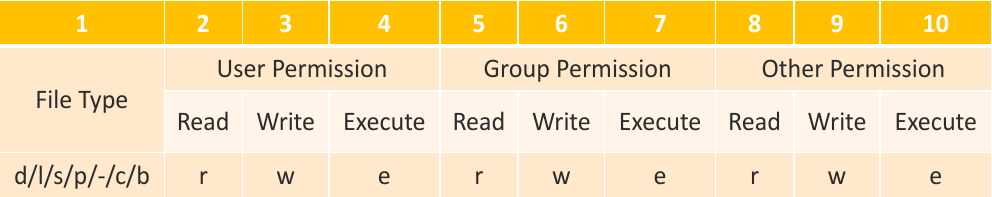
\includegraphics[width=0.6in]{images/content/1.3_file.png}
\captionof{figure}{文件描述符}
\label{fig:文件描述符}
\end{figure}

\subsubsection{字节序}
\indent \setlength{\parindent}{2em}

\indent 目前计算机中采用两种字节存储机制:大端(Big-endian)和小端(Little-endian)。

\indent Big-endian 规定 MSB 在存储时放在低地址,在传输时放在流的开始;LSB 存储时放在高地址,在传输时放在流的末尾。Little-endian 则相反。

\indent 常见的 Intel 处理器使用 Little-endian,而 PowerPC 系列处理器则使用 Big-endian,另外 TCP/IP 协议和 Java 虚拟机的字节序也是 Big-endian。

\indent 例如十六进制整数 \verb+0x12345678+ 存入以 \verb+1000H+ 开始的内存中:
\indent \ \\
\indent \ \\
\indent \ \\
\indent \ \\
\indent \ \\
\indent \ \\
\indent \ \\
\begin{figure}[ht]
    \indent \\
    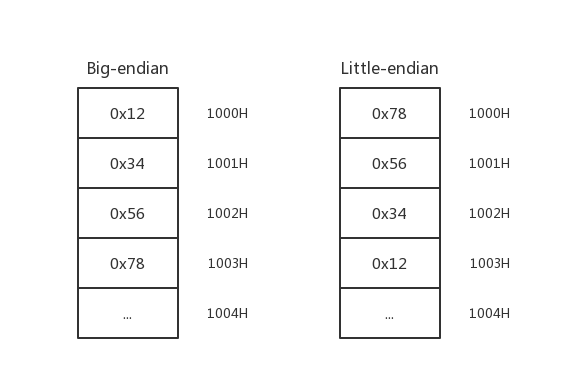
\includegraphics[width=0.8in]{images/content/1.3_byte_order.png}
    \captionof{figure}{字节序}
    \label{fig:字节序}
\end{figure}
\indent \\
\indent 我们在内存中实际地看一下,在地址 \verb+0xffffd584+ 处有字符 \verb+1234+,在地址 \verb+0xffffd588+处有字符 \verb+5678+。
\begin{lstlisting}[language=bash, style=customStyleBashDark, caption=内存中的字节]
gdb-peda$ x/w 0xffffd584
0xffffd584:     0x34333231
gdb-peda$ x/4wb 0xffffd584
0xffffd584:     0x31    0x32    0x33    0x34
gdb-peda$ python print('\x31\x32\x33\x34')
1234

gdb-peda$ x/w 0xffffd588
0xffffd588:     0x38373635
gdb-peda$ x/4wb 0xffffd588
0xffffd588:     0x35    0x36    0x37    0x38
gdb-peda$ python print('\x35\x36\x37\x38')
5678

gdb-peda$ x/2w 0xffffd584
0xffffd584:     0x34333231      0x38373635
gdb-peda$ x/8wb 0xffffd584
0xffffd584:     0x31    0x32    0x33    0x34    0x35    0x36    0x37    0x38
gdb-peda$ python print('\x31\x32\x33\x34\x35\x35\x36\x37\x38')
123455678
db-peda$ x/s 0xffffd584
0xffffd584:     "12345678"
\end{lstlisting}

\subsubsection{输入输出}
\indent \setlength{\parindent}{2em}
\begin{itemize}
    \item 使用命令的输出作为可执行文件的输入参数
    \item \verb|$ ./vulnerable 'your_command_here'|
    \item \verb|$ ./vulnerable $(your_command_here)|
    \item 使用命令作为输入
    \item \verb+$ your_command_here | ./vulnerable+
    \item 将命令行输出写入文件
    \item \verb+$ your_command_here > filename+
    \item 使用文件作为输入
    \item \verb+$ ./vulnerable < filename+
\end{itemize}

\subsubsection{文件描述符}
\indent \setlength{\parindent}{2em}

\indent 在 Linux 系统中一切皆可以看成是文件,文件又分为:普通文件、目录文件、链接文件和设备文件。文件描述符(file descriptor)是内核管理已被打开的文件所创建的索引,使用一个非负整数来指代被打开的文件。

\indent 标准文件描述符如下:

\indent 当一个程序使用 \verb+fork()+ 生成一个子进程后,子进程会继承父进程所打开的文件表,此时,父子进程使用同一个文件表,这可能导致一些安全问题。如果使用 \verb+vfork()+,子进程虽然运行于父进程的空间,但拥有自己的进程表项。

\subsubsection{核心转储}
\indent \setlength{\parindent}{2em}

\subsubsection{调用约定}
\indent \setlength{\parindent}{2em}

\subsubsection{环境变量}
\indent \setlength{\parindent}{2em}

\subsubsection{/proc/[pid]}
\indent \setlength{\parindent}{2em}

\section{Web安全基础}
\indent \setlength{\parindent}{2em}

\section{逆向工程基础}
\indent \setlength{\parindent}{2em}

\section{现代密码学基础}
\indent \setlength{\parindent}{2em}

\section{Android安全基础}
\indent \setlength{\parindent}{2em}
